\chapter{Метрические методы}

\section{Постановка задачи метрического обучения}
Пусть $\mathbf{X} = [\bx_1, \ldots, \bx_N] \in \mathbb{R}^{T \times N}$~--- множество объектов.
Объект $\mathbf{x}_i = [x_i^1, \ldots, x_i^T]^\top$ задан в виде вектора в пространстве признаков.
Требуется выявить кластерную структуру данных и разбить множество объектов $\mathbf{X}$ на множество непересекающихся кластеров,
т.\,е.\ построить отображение
\[
a: \mathbf{X} \to \{1, \dots, K\}.
\]
Обозначим $y_i = a (\bx_i)$, $y_i \in \{1, \ldots, K\}$,~--- метка кластера объекта $\bx_i$.
Необходимо выбрать метки кластеров $\{y_i\}_{i=1}^N$ таким образом, чтобы расстояния между кластерами были максимальными.
Центр $\boldsymbol{\mu}$ множества объектов $\mathbf{X}$ и центры кластеров $\{\boldsymbol{\mu}_k\}_{k=1}^K$ вычисляются по формулам:
\begin{equation}
\label{mu}
\boldsymbol{\mu} =\frac1N \sum_{i=1}^N\bx_i\,; \quad
\boldsymbol{\mu}_k =\frac{ \sum_{i=1}^N [y_i = y_k]\mathbf{x}_i } {\sum_{i=1}^N [y_i = y_k]}\,.
\end{equation}
Введем на множестве объектов $\mathbf{X}$ расстояние Махаланобиса
\begin{equation}
\label{metric}
\rho (\bx_i, \bx_j) = \sqrt{(\bx_i - \bx_j)^{\top} \mathbf{A}^{-1} (\bx_i - \bx_j)}\,,
\end{equation}
где $\mathbf{A}$~--- это матрица ковариаций множества $\mathbf{X}$
\begin{equation}
\label{covMatrix}
\mathbf{A} = \frac 1N \sum_{i=1}^N(\bx_i - \boldsymbol{\mu})(\bx_i - \boldsymbol{\mu})^{\top}.
\end{equation}
\begin{definition}
	Функционалом качества кластеризации $Q$ назовем межкластерное расстояние:
	\[
	Q (\{\boldsymbol{\mu}_k\}_{k=1}^K)= \sum_{k=1}^K N_k \rho^2(\boldsymbol{\mu}_k, \boldsymbol{\mu})\,,
	\]
	где $N_k = \sum_{i=1}^N [y_i = y_k]$~--- число объектов в кластере $k$.
\end{definition}

Поставим задачу кластеризации как задачу максимизации функционала
\begin{equation}
\label{Qmax}
Q \bigl(\{\boldsymbol{\mu}_k\}_{k=1}^K\bigr) \to \max_{\boldsymbol{\mu}_k \in \mathbb{R}^T}.
\end{equation}
Для улучшения качества решения этой задачи предлагается применить метод метрического обучения к ковариационной матрице $\mathbf{A}$.
Найдем такую матрицу $\mathbf{A}$, для которой функционал качества принимает максимальное значение:
\begin{equation}
\label{Amax}
\mathbf{A}^* = \mathop{\arg \max}_{\mathbf{A} \in \mathbb{R}^{T \times T}} Q \bigl(\{\boldsymbol{\mu}_k^*\}_{k=1}^K \bigr)\,,
\end{equation}
где $\{\boldsymbol{\mu}_k^*\}_{k=1}^K$~--- решение задачи кластеризации~(\ref{Qmax}).

\section{Алгоритм адаптивного метрического обучения}
Для решения поставленных оптимизационных задач~(\ref{Qmax}), (\ref{Amax}) используется алгоритм адаптивного метрического обучения.
Предлагается понизить размерность пространства объектов $\mathbf{X}$ с помощью линейного ортогонального преобразования $\mathbf{G} \in \mathbb{R}^{T \times L}$, $\mathbf{G}^{\top} \mathbf{G} = \mathbf{I}$, где новая размерность $L < T$
\[
\mathbf{X} \ni \bx_i  \mapsto \hat{\bx}_i = \mathbf{G}^\top \bx_i \in \mathbb{R}^L, \quad i = 1, \ldots, N.
\]
Центр $\hat{\boldsymbol{\mu}}$ множества объектов $\{\hat{\bx}_i\}_{i=1}^N$ вычисляется по формуле~(\ref{mu}). Расстояния между объектами вычисляются по формуле~(\ref{metric}), где в качестве матрицы $\hat{\mathbf{A}}$ используется матрица ковариаций~(\ref{covMatrix}) множества объектов $\{\hat{\bx}_i\}_{i=1}^N$

\[
\hat{\mathbf{A}} =
\frac 1N \sum_{i=1}^N (\hat{\bx}_i - \hat{\boldsymbol{\mu}})(\hat{\bx}_i - \hat{\boldsymbol{\mu}})^\top =
\frac 1N \sum_{i=1}^N \mathbf{G}^{\top}(\bx_i - \boldsymbol{\mu})(\bx_i - \boldsymbol{\mu})^\top \mathbf{G} =  \mathbf{G}^{\top} \mathbf{A} \mathbf{G}.
\]
\begin{definition}
	Индикаторной матрицей назовем матрицу $\mathbf{F} = \{\delta_{ik}\} \in \mathbb{R}^{N \times K}$, где
	\[
	\delta_{ik} =
	\begin{cases}
	1, & \text{если $a(\bx_i) = y_k$;} \\
	0, & \text{если $a(\bx_i) \neq y_k$.}
	\end{cases}
	\]
\end{definition}
\begin{definition}
	Взвешенной индикаторной матрицей назовем матрицу
	$\mathbf{L} = \mathbf{F} (\mathbf{F}^{\top} \mathbf{F})^{-1/2} = \{l_{ik}\} \in \mathbb{R}^{N \times K}$, элементы которой равны:
	\[
	l_{ik} =
	\begin{cases}
	\displaystyle    \frac 1{\sqrt{N_k}}, & \text{если $a(\bx_i) = y_k$;} \\
	0, & \text{если $a(\bx_i) \neq y_k$.}
	\end{cases}
	\]
\end{definition}
\begin{theorem}
	C использованием данных обозначений задача кластеризации~(\ref{Qmax})
	и~задача метрического обучения~(\ref{Amax}) сводятся к общей задаче максимизации функционала качества~\cite{ding2005equivalence}
	\begin{equation}
	\label{GLmax}
	Q = \frac 1N \text{trace} (\mathbf{L}^{\top} \mathbf{X}^{\top} \mathbf{G} \hat{\mathbf{A}}^{-1} \mathbf{G}^{\top} \mathbf{X L}) = \frac 1N \text{trace} (\mathbf{L}^{\top} \mathbf{X}^{\top} \mathbf{G}
	(\mathbf{G}^{\top} \mathbf{A G})^{-1} \mathbf{G}^{\top} \mathbf{X L}) \to \max_{\mathbf{G}, \mathbf{L}}.
	\end{equation}
\end{theorem}
\section{Решение задачи метрического обучения}
Для решения задачи~(\ref{GLmax}) алгоритм адаптивного метрического обучения использует \mbox{EM-под}\-ход.
На каждом шаге итеративно вычисляются локальные оптимальные значения матриц $\mathbf{G}$ и $\mathbf{L}$.
На $E$-шаге необходимо найти матрицу $\mathbf{L}$, которая является решением оптимизационной задачи~(\ref{GLmax}) при фиксированной матрице $\mathbf{G}$.
В качестве начального приближения получим взвешенную индикаторную матрицу $\mathbf{L}$ с помощью алгоритма кластеризации $k$-средних с евклидовой метрикой.
На $M$-шаге производится нахождение оптимального значения матрицы $\mathbf{G}$ при фиксированной матрице $\mathbf{L}$.
Алгоритм завершается при стабилизации функционала $Q$ на последовательности итераций.

\subsection{Алгоритм $k$-средних}
В данной работе базовым алгоритмом для сравнения является алгоритм $k$-средних.
Первым шагом алгоритм выбирает из множества $\mathbf{X}$ случайным образом $K$ объектов $\{\boldsymbol{\mu}_k\}_{k=1}^K$~--- начальные центры кластеров.
Для каждого объекта $\bx_i$ вычисляется расстояние~(\ref{metric}) до каждого центра кластера $\boldsymbol{\mu}_k$ с единичной матрицей трансформаций.
Объект~$\bx_i$ относится к кластеру, расстояние до которого оказалось наименьшим.
Далее производится вычисление новых центров кластеров по формуле~(\ref{mu}).
Алгоритм завершается, если значения центров кластеров прекращают меняться.

\subsection{Оптимизация матрицы G с фиксированной матрицей L}
Для любых двух квадратных матриц $\mathbf{A}$ и $\mathbf{B}$ справедливо $\text{trace}(\mathbf{AB}) = \text{trace}(\mathbf{BA})$.
Данное свойство позволяет переформулировать задачу~(\ref{GLmax}) следующим образом:
\[
Q = \frac 1N \text{trace} (\mathbf{L}^{\top} \mathbf{X}^{\top} \mathbf{G} (\mathbf{G}^{\top} \mathbf{A G})^{-1} \mathbf{G}^{\top} \mathbf{X L}) = \frac 1N \text{trace} \bigl((\mathbf{G}^{\top} \mathbf{A G})^{-1} \mathbf{G}^{\top} \mathbf{X L L}^{\top} \mathbf{X}^{\top} \mathbf{G}\bigr).
\]
\begin{theorem}
	Обозначим $\mathbf{B} = \mathbf{X L L}^{\top} \mathbf{X}^{\top}$.
	Обозначим через $\mathbf{G} = [\mathbf{v}_1, \ldots, \mathbf{v}_K]$ матрицу, состоящую из $K$ собственных векторов матрицы $\mathbf{A}^{-1}\mathbf{B}$, отвечающих наибольшим собственным значениям.
	Тогда решением~(\ref{GLmax}) является ортогональная матрица, полученная $QR$-раз\-ло\-же\-ни\-ем матрицы $\mathbf{G}$.
\end{theorem}

Функционал качества $Q$ зависит только от матрицы $\mathbf{G}$. Обозначим
\[
s(\mathbf{G}) = \text{trace} \bigl((\mathbf{G}^{\top} \mathbf{A G})^{-1} \mathbf{G}^{\top} \mathbf{B G}\bigr).
\]
На данном шаге задача~(\ref{GLmax}) принимает вид:
\begin{gather}
\label{Gmax}
\mathbf{G}^* = \mathop{\arg \max}_{\mathbf{G} \in \mathbb{R}^{T \times L}} s(\mathbf{G})\,; \\
\label{Gorth}
\mathbf{G}^{\top} \mathbf{G} = \mathbf{I}\,.
\end{gather}
Ранг произведения матриц не превосходит рангов сомножителей, поэтому ранг матрицы~$\mathbf{B}$ не превосходит $K$.
Решением~(\ref{Gmax}) является матрица $\mathbf{G} = [\mathbf{v}_1, \ldots, \mathbf{v}_K]$, состоящая
из~$K$~собственных векторов матрицы $\mathbf{A}^{-1}\mathbf{B}$, отвечающих наибольшим собственным значениям.
Таким образом, размерность нового пространства объектов будет равна количеству кластеров $K$.

В общем случае матрица $\mathbf{G}$ не является ортогональной.
Заметим, что для любой невырожденной матрицы $\mathbf{G}$ верно $s(\mathbf{G}) = s(\mathbf{G M})$.
Для учета условия ортогональности~(\ref{Gorth}) найдем $QR$-разложение матрицы $\mathbf{G}$.
Тогда ортогональная матрица $\mathbf{Q}$ является оптимальным значением $\mathbf{G}^*$.

\subsection{Оптимизация матрицы L с фиксированной матрицей G}
\begin{theorem}
	Обозначим $\hat{\mathbf{K}} = (1/N)\mathbf{X}^{\top} \mathbf{G} \hat{\mathbf{A}}^{-1} \mathbf{G}^{\top} \mathbf{X}$.
	Тогда задача~(\ref{GLmax}) эквивалентна задаче кластеризации $k$-средних с заданным ядром $\hat{\mathbf{K}}$~\cite{shawe2004kernel}.
\end{theorem}

При фиксированной матрице $\mathbf{G}$ задача~(\ref{GLmax}) принимает вид:
\begin{equation*}
%\label{Lmax}
\text{trace} (\mathbf{L}^{\top} \hat{\mathbf{K}} \mathbf{L}) \to \max_{\mathbf{L} \in \mathbb{R}^{N \times K}}.
\end{equation*}
Матрица $\hat{\mathbf{K}}$ является симметричной и неотрицательно определенной, тем самым может быть выбрана в качестве ядра.



\section{Постановка задачи}
Пусть объект $\mathbf{x}_i \in \mathbb{R}^n$~--- временной ряд, последовательность измерений некоторой исследуемой величины в различные моменты времени.
Пусть $\mathbf{X}$~--- множество всех временных рядов фиксированной длины $n$, $Y = \{1, \dots, K\}$~--- множество меток классов.
Пусть задана выборка $\mathfrak{D} = \{(\mathbf{x}_i, y_i)\}_{i=1}^\ell$~--- множество объектов с известными метками классов $y_i \in Y$.

Требуется построить точную, простую, устойчивую модель классификации
\[
a: \mathbf{X} \to Y.
\]
Данную модель представим в виде суперпозиции
\begin{equation}
\label{eq:classifiers}
a(\mathbf{x}) = b \circ \mathbf{f} \circ G(\mathbf{x}, \{\mathbf{c}_e\}_{e = 1} ^ K),
\end{equation}
где $G$~--- процедура выравнивания временных рядов относительно центроидов классов~$\{\mathbf{c}_e\}_{e = 1} ^ K$, $\mathbf{f}$~--- алгоритм метрического обучения, $b$~--- алгоритм многоклассовой классификации.

\subsection{Выравнивание временных рядов.}

Для повышения качества и устойчивости алгоритма классификации предлагается провести выравнивание временных рядов каждого класса относительно центроида.

Пусть $\mathbf{X}_e$ --- множество объектов обучающей выборки $\mathfrak{D}$, принадлежащих одному классу $e \in \{1, \dots, K\}$.
Центроидом множества объектов $\mathbf{X}_e = \{\mathbf{x}_i|y_i=e\}_{i=1}^\ell$ по расстоянию $\rho$ назовем вектор $\mathbf{c}_e \in \mathbb{R}^n$ такой, что
\begin{equation}
\label{centroid_task}
\mathbf{c}_e = \mathop{\text{argmin}}\limits_{{\mathbf{c} \in \mathbb{R}^n}}\sum_{\mathbf{x}_i \in \mathbf{X}_e}
{\rho(\mathbf{x}_i ,\mathbf{c})}.
\end{equation}

Для нахождения центроида предлагается в качестве расстояния между временными рядами использовать путь наименьшей стоимости~\cite{goncharov2015cost}, найденный методом динамической трансформации времени.
Псевдокод решения оптимизационной задачи~(\ref{centroid_task}) приведен в алгоритме~\ref{DBA_pseudo}.

\begin{algorithm}
	\caption{Нахождение центроида $\text{DBA}(\mathbf{X}_e, \text{n\_iter})$}
	\label{DBA_pseudo}
	\begin{algorithmic}[1]
		\REQUIRE $\mathbf{X}_e$~--- множество временных рядов, принадлежащих одному и тому же классу, n\_iter~--- количество итераций алгоритма.
		\ENSURE $\mathbf{c}$~--- центроид множества $\mathbf{X}_e$.
		
		\STATE {задать начальное приближение приближение центроида $\mathbf{c}$;}
		\FOR {$i = 1, \dots, \text{n\_iter}$}
		\FOR {$\mathbf{x} \in \mathbf{X}_e$}
		\STATE{вычислить выравнивающий путь между $\mathbf{c}$ и $\mathbf{x}$}
		\STATEx $ \quad \quad \text{alignment}(\mathbf{x}) := \text{DTWalignment}(\mathbf{c}, \mathbf{x})$;
		\ENDFOR
		\STATE {объединить поэлементно множества индексов для каждого отсчета времени}
		\STATEx {$ \quad \text{alignment} := \bigcup_{\mathbf{x} \in \mathbf{X}_e} \text{alignment}(\mathbf{x})$};
		\STATE {$\mathbf{c} = \text{mean}(\text{alignment})$}
		\ENDFOR
	\end{algorithmic}

	\textbf{DTWalignment}($\mathbf{c}$, $\mathbf{x}$)
	\begin{algorithmic}[1]
		\REQUIRE $\mathbf{c}, \mathbf{x}$~--- временные ряды.
		\ENSURE alignment~--- выравнивающий путь.\COMMENT {каждый индекс временного ряда~$\mathbf{x}$ поставлен в однозначное соответствие индексу временного ряда~$\mathbf{c}$}
		
		\STATE {построить $n \times n$-матрицу деформаций DTW}
		\STATEx {$\text{cost} := \text{DTW}(\mathbf{c}, \mathbf{x})$};
		
		\STATE {вычислить выравнивающий путь по матрице деформаций}
		\STATEx {$\text{alignment} := \text{DTWpath}(\text{cost})$};
	\end{algorithmic}
\end{algorithm}
\newpage
Общая процедура выравнивания имеет следующий вид:
\begin{itemize}
	\item[1)]
	построить множество центроидов классов $\{\mathbf{c}_e\}_{e = 1}^K$;
	\item[2)]
	по множеству центроидов найти пути наименьшей стоимости между каждым
	временным рядом $\mathbf{x}_i$ и центроидом его класса $\mathbf{c}_{y_i}$;
	\item[3)]
	по каждому пути восстановить выравненный временной ряд;
	\item[4)]
	привести множества выравненных временных рядов к нулевому среднему и нормировать на дисперсию.
\end{itemize}

Результатом выравнивания должно стать множество выравненных временных рядов.

\subsection{Метрическое обучение.}

Введем на множестве выравненных временных рядов расстояние Махаланобиса
\[
d_\mathbf{A} (\mathbf{x}_i, \mathbf{x}_j) = \sqrt{(\mathbf{x}_i - \mathbf{x}_j)^\mathsf{T} \mathbf{A} (\mathbf{x}_i - \mathbf{x}_j)},
\]
где матрица трансформаций $\mathbf{A} \in \bbR^{n \times n}$ является симметричной и неотрицательно определенной ($\mathbf{A}^\mathsf{T} = \mathbf{A}$, $\mathbf{A} \succeq 0$).
Представим матрицу $\mathbf{A}$ в виде разложения $\mathbf{A} = \mathbf{L}^\mathsf{T}  \mathbf{L}$.
Матрица $\mathbf{L} \in \bbR^{p \times n}$~--- матрица линейного преобразования, где $p$ задает размерность преобразованного пространства. Если параметр $p < n$, то происходит снижение размерности признакового пространства.

Расстояние $d_\mathbf{A} (\mathbf{x}_i, \mathbf{x}_j)$ есть евклидово расстояние между $\mathbf{Lx}_i$ и $\mathbf{Lx}_j$:
\[
d_\mathbf{A} (\mathbf{x}_i, \mathbf{x}_j) = \sqrt{(\mathbf{x}_i - \mathbf{x}_j)^\mathsf{T} \mathbf{L}^\mathsf{T} \mathbf{L} (\mathbf{x}_i - \mathbf{x}_j)} = \sqrt{(\mathbf{L} (\mathbf{x}_i - \mathbf{x}_j))^\mathsf{T} (\mathbf{L} (\mathbf{x}_i - \mathbf{x}_j))} = \|\mathbf{L} (\mathbf{x}_i - \mathbf{x}_j)\|_2.
\]

В качестве алгоритма метрического обучения в данной работе был выбран алгоритм LMNN. Данный алгоритм сочетает в себе идеи метода $k$ ближайших соседей. Первая идея заключается в минимизации расстояний между $k$ ближайшими объектами, находящимися в одном классе. Запишем функционал качества в виде
\[
Q_1(\mathbf{L}) = \sum_{j \rightsquigarrow i} \|\mathbf{L}(\mathbf{x}_i - \mathbf{x}_j)\|^2 \rightarrow \min_{\mathbf{L}},
\]
где $j \rightsquigarrow i$ означает, что $\mathbf{x}_j$ является одним из $k$ ближайших соседей для $\mathbf{x}_i$.
Вторая идея состоит в максимизации расстояния между каждым объектом и его объектами-нарушителями. Объектом-нарушителем для $\mathbf{x}_i$ назовем объект $\mathbf{x}_l$ такой, что
\begin{equation}
\label{impostor}
\|\mathbf{L}(\mathbf{x}_i - \mathbf{x}_l)\|^2 \leq \|\mathbf{L}(\mathbf{x}_i - \mathbf{x}_j)\|^2 + 1, \quad \text{где $j \rightsquigarrow i$}.
\end{equation}
Таким образом, необходимо минимизировать следующий функционал:
\[
Q_2(\mathbf{L}) = \sum_{j \rightsquigarrow i} \sum_l(1 - y_{il})\bigl[1 + \|\mathbf{L}(\mathbf{x}_i - \mathbf{x}_j)\|^2 - \|\mathbf{L}(\mathbf{x}_i - \mathbf{x}_l)\|^2\bigr]_+ \rightarrow \min_{\mathbf{L}},
\]
где $y_{il} = 1$, если $y_i = y_l$, и $y_{il} = 0$ в противном случае.
Положительная срезка позволяет штрафовать только те объекты, которые удовлетворяют условию~(\ref{impostor}).

Задача метрического обучения состоит в нахождении линейного преобразования $\mathbf{f}(\mathbf{x}) = \mathbf{Lx}$, то есть нахождении матрицы $\mathbf{L}$ в виде решения оптимизационной задачи
\begin{equation}
\label{Qmin}
Q(\mathbf{L}) = \mu Q_1(\mathbf{L}) + (1 - \mu) Q_2(\mathbf{L}) \rightarrow \min_{\mathbf{L}},
\end{equation}
где $\mu \in (0, 1)$~--- весовой параметр, определяющий вклад каждого из функционалов.
Задача~(\ref{Qmin}) представляет собой задачу полуопределенного программирования~\cite{vandenberghe1996semidefinite} и может быть решена существующими оптимизационными пакетами.

\subsection{Классификация временных рядов.}

Пусть $\mathbf{x} \in \mathbf{X}$~--- неразмеченный временной ряд. Выравниваем временной ряд $\mathbf{x}$ относительно всех центроидов классов
\[
\mathbf{\hat{x}}_e = G(\mathbf{x}, \mathbf{c}_e), \quad \text{где} \quad e = \{1, \dots, K\}.
\]
Отнесем временной ряд к классу, для которого минимально расстояние до соответствующего центроида. В качестве расстояния используем обученную метрику Махаланобиса с фиксированной матрицей $\mathbf{A}$
\[
\hat{y} = \mathop{\text{argmin}}\limits_{e \in \{1, \dots, K\}}d_\mathbf{A}(\mathbf{\hat{x}}_e, \mathbf{c}_e).
\]
После нахождения оптимальных центроидов классов и нахождения оптимальной матрицы трансформаций процедура классификации заключается в измерении расстояния между найденными центроидами и новыми неразмеченными объектами.

Для оценки качества работы алгоритма будем вычислять ошибку классификации как долю неправильно классифицированных объектов тестовой выборки $\mathfrak{U}$:
\[
\text{error} = \frac1{|\mathfrak{U}|} \sum_{i = 1} ^ {|\mathfrak{U}|} [a(\mathbf{x}_i) \ne y_i].
\]


\section{Вычислительный эксперимент}
В целях проверки работоспособности предложенного подхода проведен вычислительный эксперимент на модельных данных. Сгенерирована выборка объектов, принадлежащих одному из двух классов, в двумерном пространстве.
Каждый объект принадлежит многомерному нормальному распределению.
На рис.~$1$ показано истинное распределение объектов, черным цветом выделены истинные центры классов и линии уровня функции распределения.


Применим к данной выборке базовый алгоритм $k$-средних.
Результат кластеризации показан на рис.~2, где черным цветом выделены найденные центры классов и линии уровня функции распределения, построенной по выборочной ковариационной матрице.

Взяв за начальное приближение результаты работы алгоритма $k$-средних,
проведем клас\-те\-ри\-за\-цию с помощью алгоритма адаптивного метрического обучения.
Результаты работы алгоритма продемонстрированы на рис.~$3$.
\begin{figure}[ht]
    \center{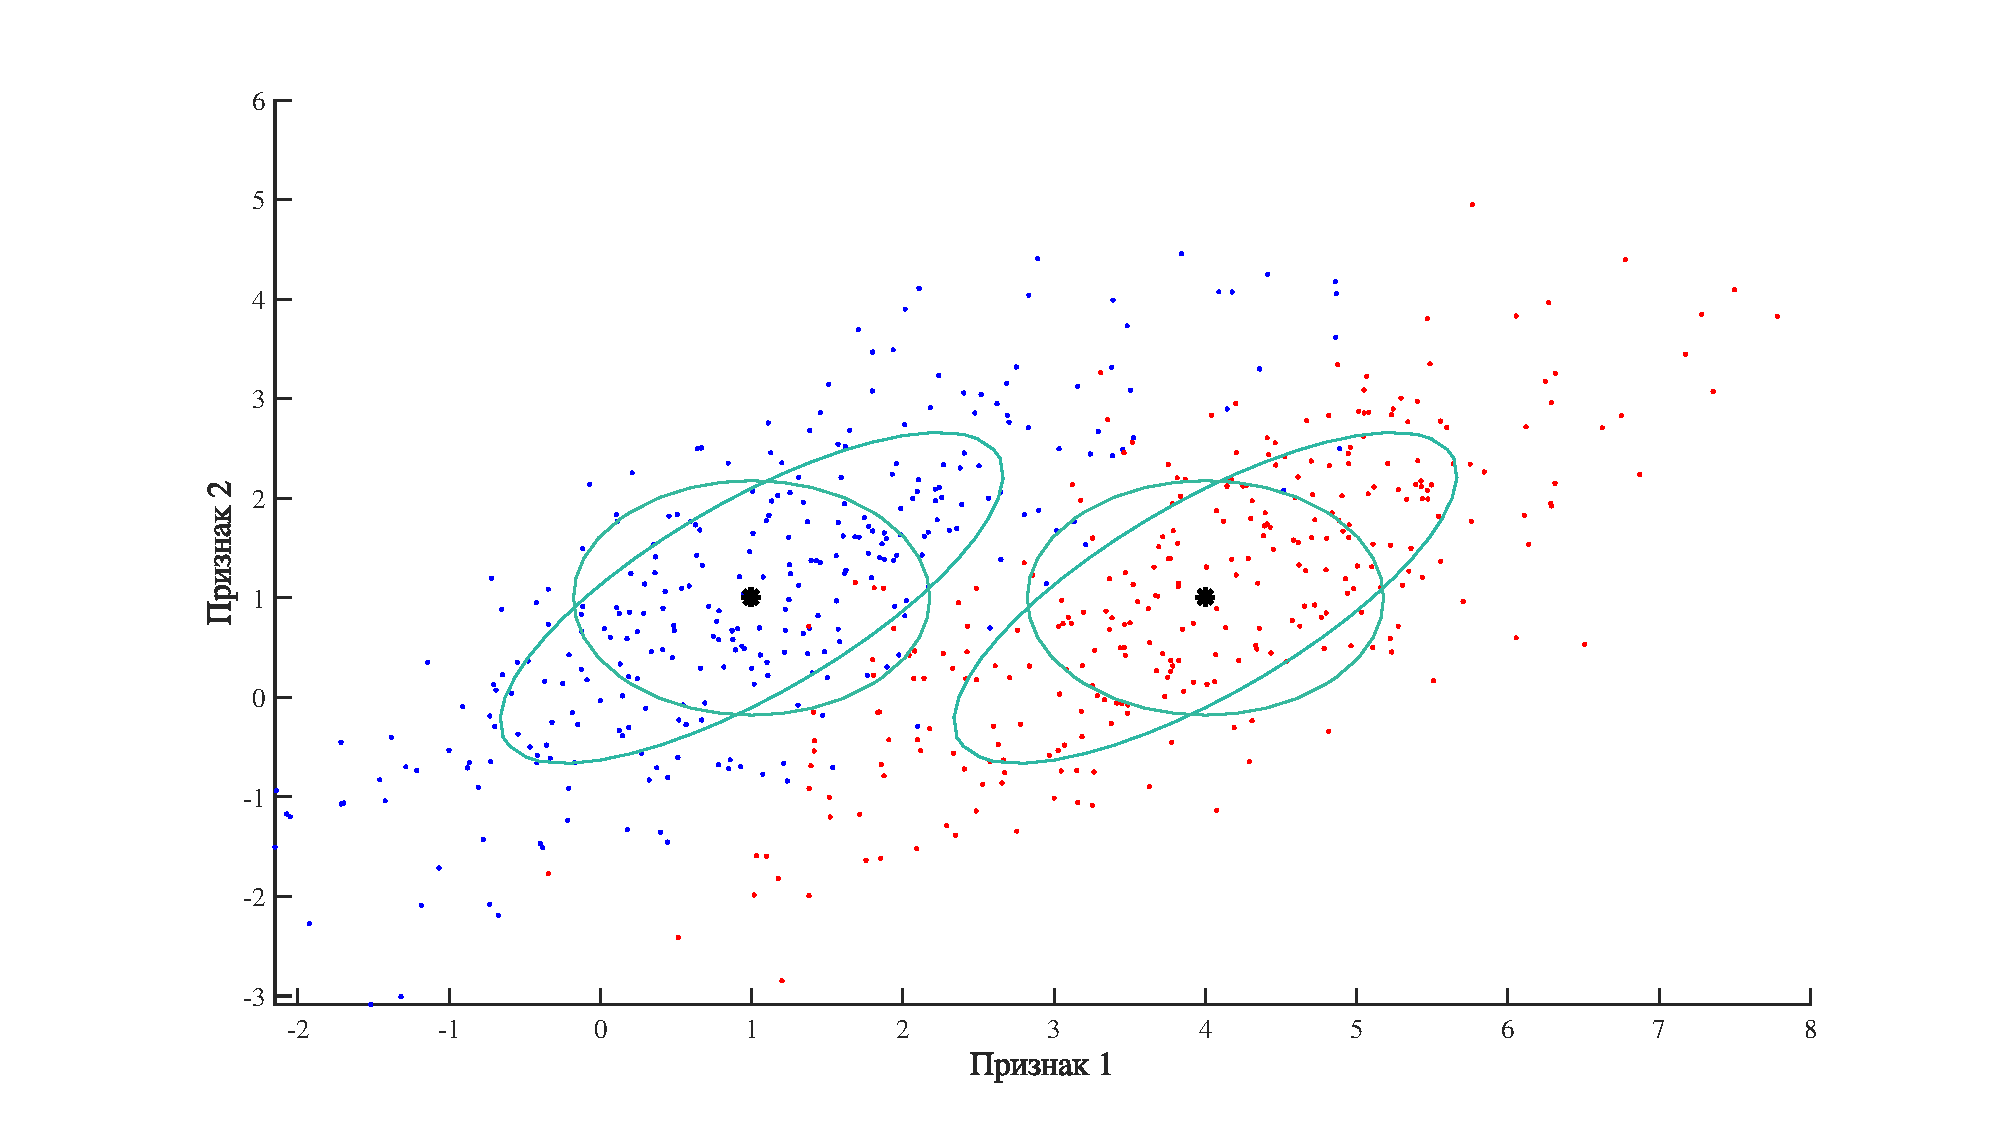
\includegraphics[width=1\linewidth]{figs/ch4/true_distribution}}
    \caption{Истинное распределение двумерных модельных данных}
\end{figure}

На рисунках заметно улучшение результатов кластеризации.
Измеренная точность кластеризации алгоритма $k$-средних составила 0,76,
алгоритма адаптивного метрического обучения~--- 0,94, что говорит о работоспособности данного подхода.
\begin{figure} %[!ht]
    \center{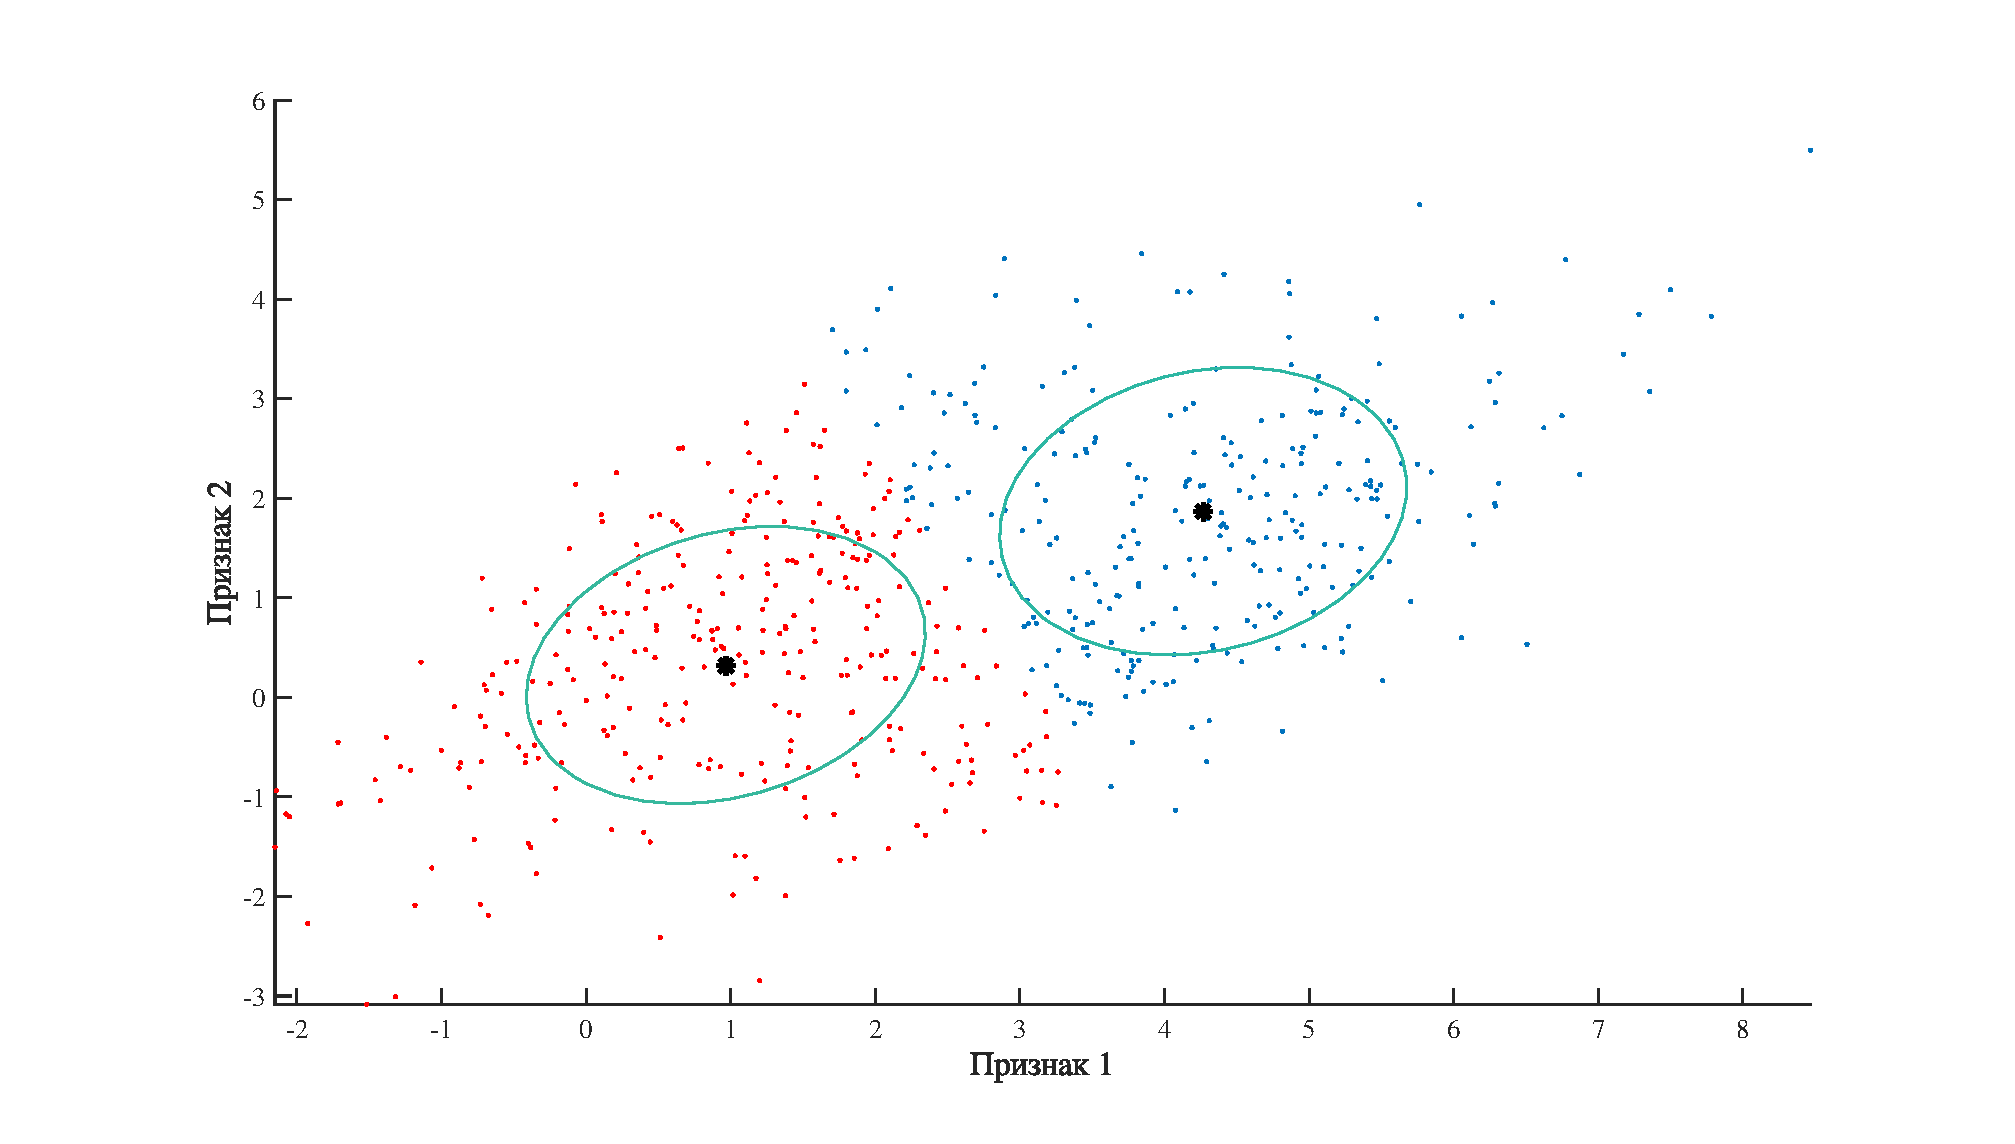
\includegraphics[width=1\linewidth]{figs/ch4/kmeans_clustering}}
    \caption{Результат кластеризации алгоритмом $k$-средних}
\end{figure}
\begin{figure} %[!ht]
    \center{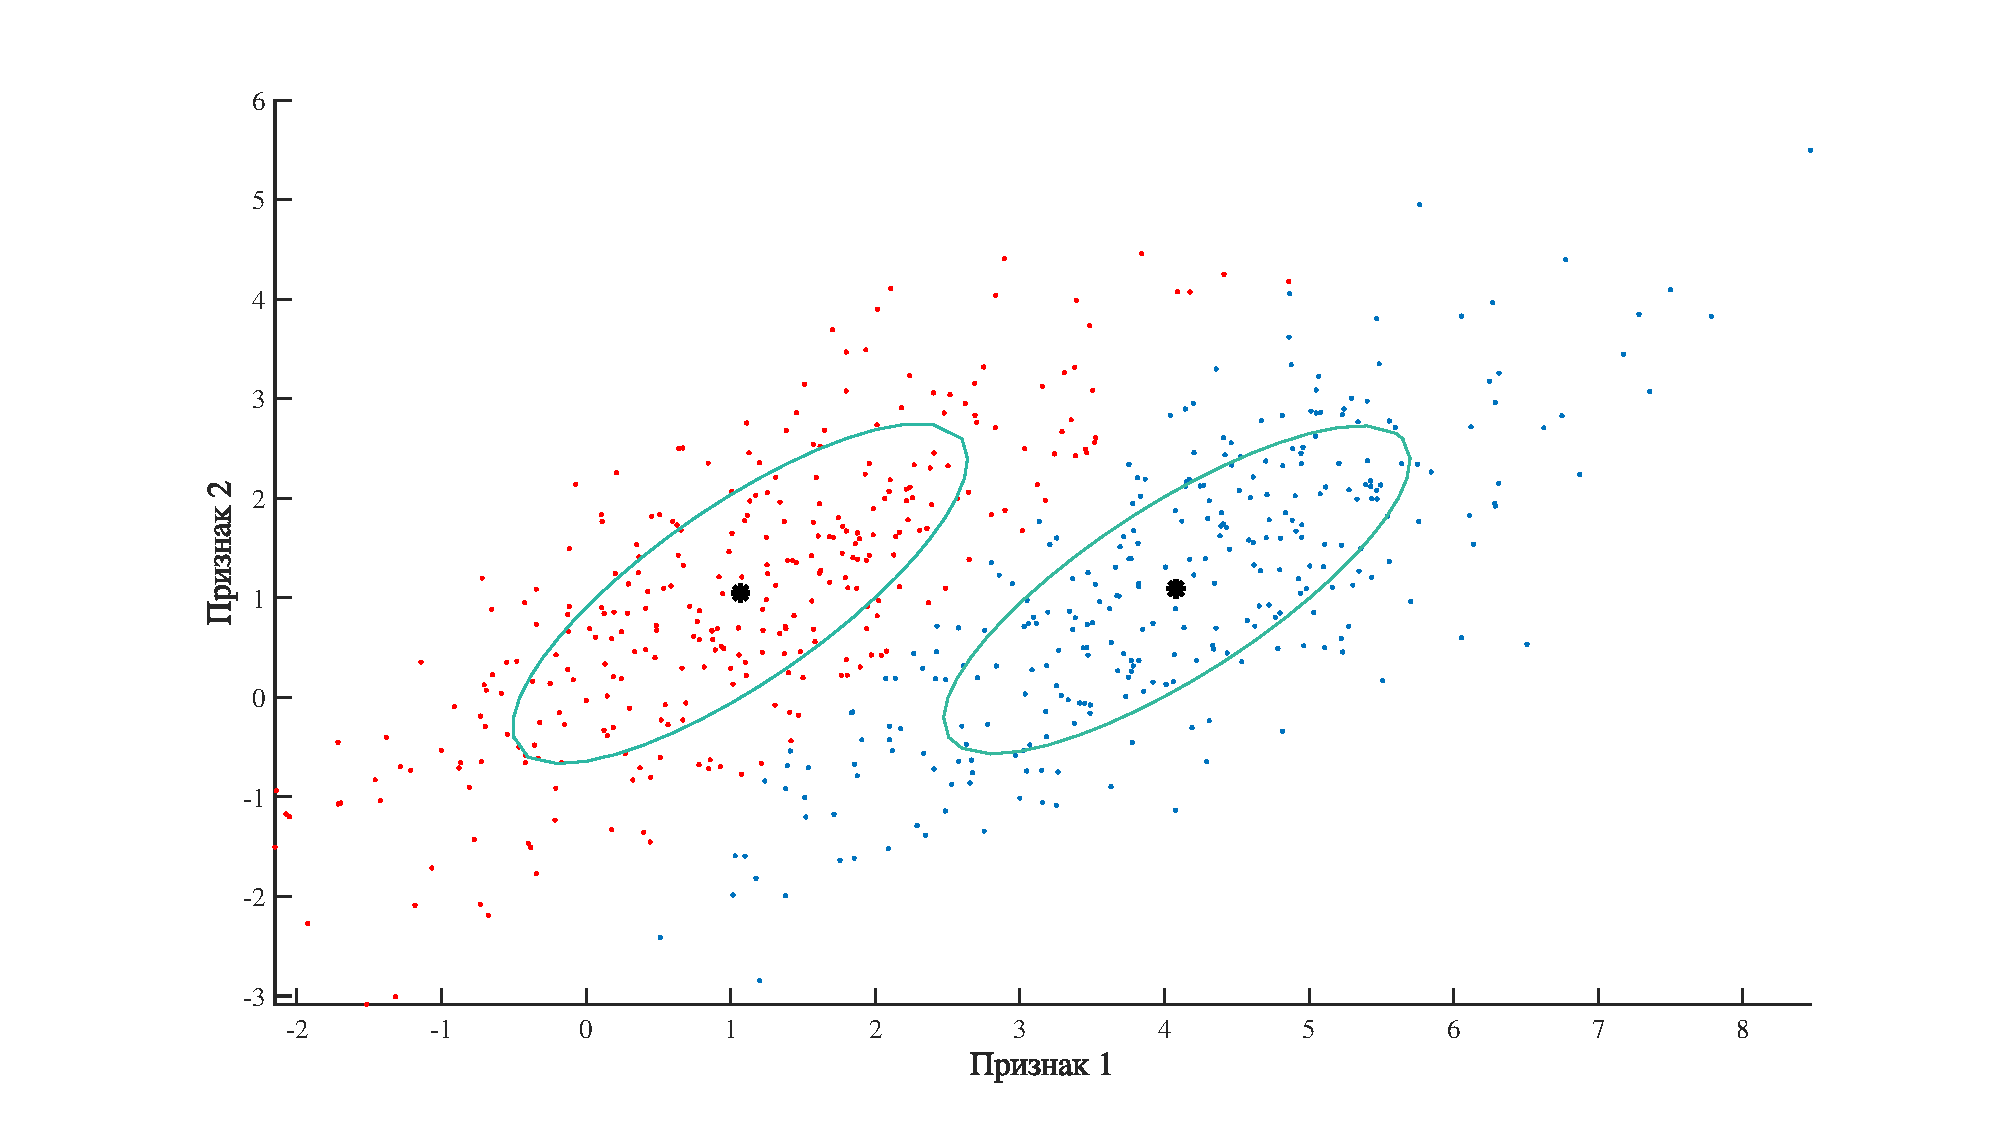
\includegraphics[width=1\linewidth]{figs/ch4/AML_clustering}}
    \caption{Результат кластеризации алгоритмом адаптивного метрического обучения}
\end{figure}


Таблица~\ref{tbl:clusteing_results} показывает результаты вычислительного эксперимента на реальных
данных.
Алгоритм был применен к $5$ выборкам, взятых из репозитория UCI~\cite{uci2017}.
Оценкой качества кластеризации служит число правильно кластеризованных объектов.
При клас\-те\-ри\-за\-ции объектов на более чем два класса возникает проблема соотнесения истинных классов с полученными кластерами.
Данная проблема была формализована в виде задачи о назначениях и решена с помощью венгерского алгоритма. Вычислительный эксперимент на реальных данных показал увеличение точности кластеризации при использовании метрического обучения.
\begin{table} %[!ht]
\centering
\caption{Результаты кластеризации}
\label{tbl:clusteing_results}

\vspace{2ex}

\begin{tabular}{|l|l|l|}
\hline
\multicolumn{1}{|c}{Выборка}                  & \multicolumn{2}{c|}{Качество кластеризации} \\ \cline{2-3}
                                          & $k$-средних               & AML                 \\
\hline
Letter Recognition                        & 0,356                 & \textbf{0,428}             \\
Optical Recognition of Handwritten Digits & 0,758                 & \textbf{0,790}               \\
Seeds                                     & 0,833                 & \textbf{0,881}            \\
Image Segmentation                        & 0,545                 & \textbf{0,737}            \\
Breast Cancer Wisconsin                   & \textbf{0,960}                 & 0,956               \\ \hline
\end{tabular}
\end{table}



	\section{Вычислительный эксперимент}
	Цель вычислительного эксперимента~--- проверить работоспособность предложенного подхода.
	Предполагается, что построенный алгоритм мультиклассовой классификации способен определить тип активности человека по форме сигнала акселерометра мобильного телефона.
	
	Для проведения базового вычислительного эксперимента были подготовлены синтетические временные ряды, принадлежащие двум классам.
	Первый класс~--- синусы вида $sin(x + b)$, где параметр $b$ определяет сдвиг каждого временного ряда.
	Второй класс~--- пилообразные функции с различными сдвигами по временной шкале.
	На каждый временной ряд был наложен нормальный шум.
	Число временных рядов каждого класса = 60.
	Длина каждого временного ряда $n = 50$.
	
	Построенные центроиды классов проиллюстрированы на рис.~\ref{centroids_synthetic}.
	Из рисунка видно, что процедура корректно определяет сдвиги временных рядов.
	\begin{figure}[ht]
		\centering
		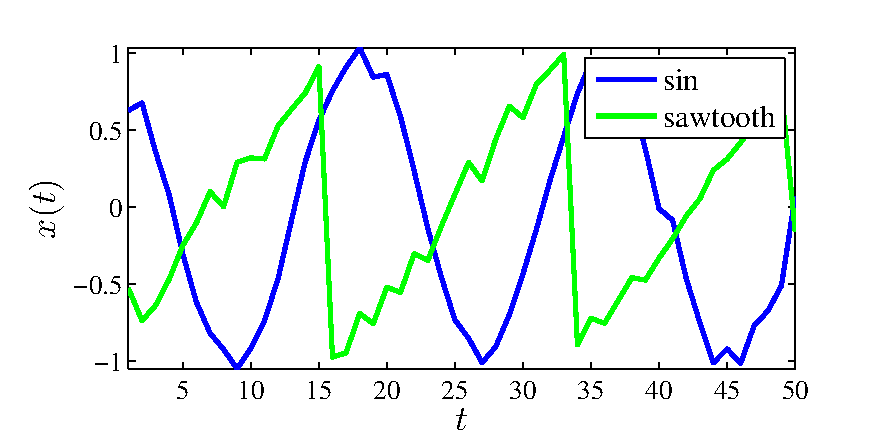
\includegraphics[width=0.45\linewidth]{figs/ch4/centroids_synthetic_noize}
		\caption{Центроиды синтетических временных рядов}
		\label{centroids_synthetic}
	\end{figure}
	
	Для того чтобы убедиться в целесообразности применения метрического обучения, данные
	временные ряды классифицировались в пространстве с евклидовой метрикой и в пространстве с метрикой Махаланобиса.
	Число ближайших соседей $k = 5$, размерность преобразованного пространства $p = 40$.
	Полученные ошибки классификации составили:
	
	евклидова метрика --- $27\%$
	
	метрика Махаланобиса --- $6\%$.
	
	Реальные данные~\cite{wisdm} представляли собой временные ряды акселерометра мобильного телефона.
	Каждый из шести классов соответствовал определенной физической активности испытуемых.
	Для проведения вычислительного эксперимента было выбрано по $200$ объектов каждого класса.
	Длина каждого временного ряда равнялась $n = 128$ отсчетам времени.
	
	Построенные центроиды классов изображены на рис.~\ref{centroids_real}.
	Найденные центроиды обладают периодичностью, свойственной временным рядам показаний активности человека.
	\begin{figure}[ht]
		\centering
		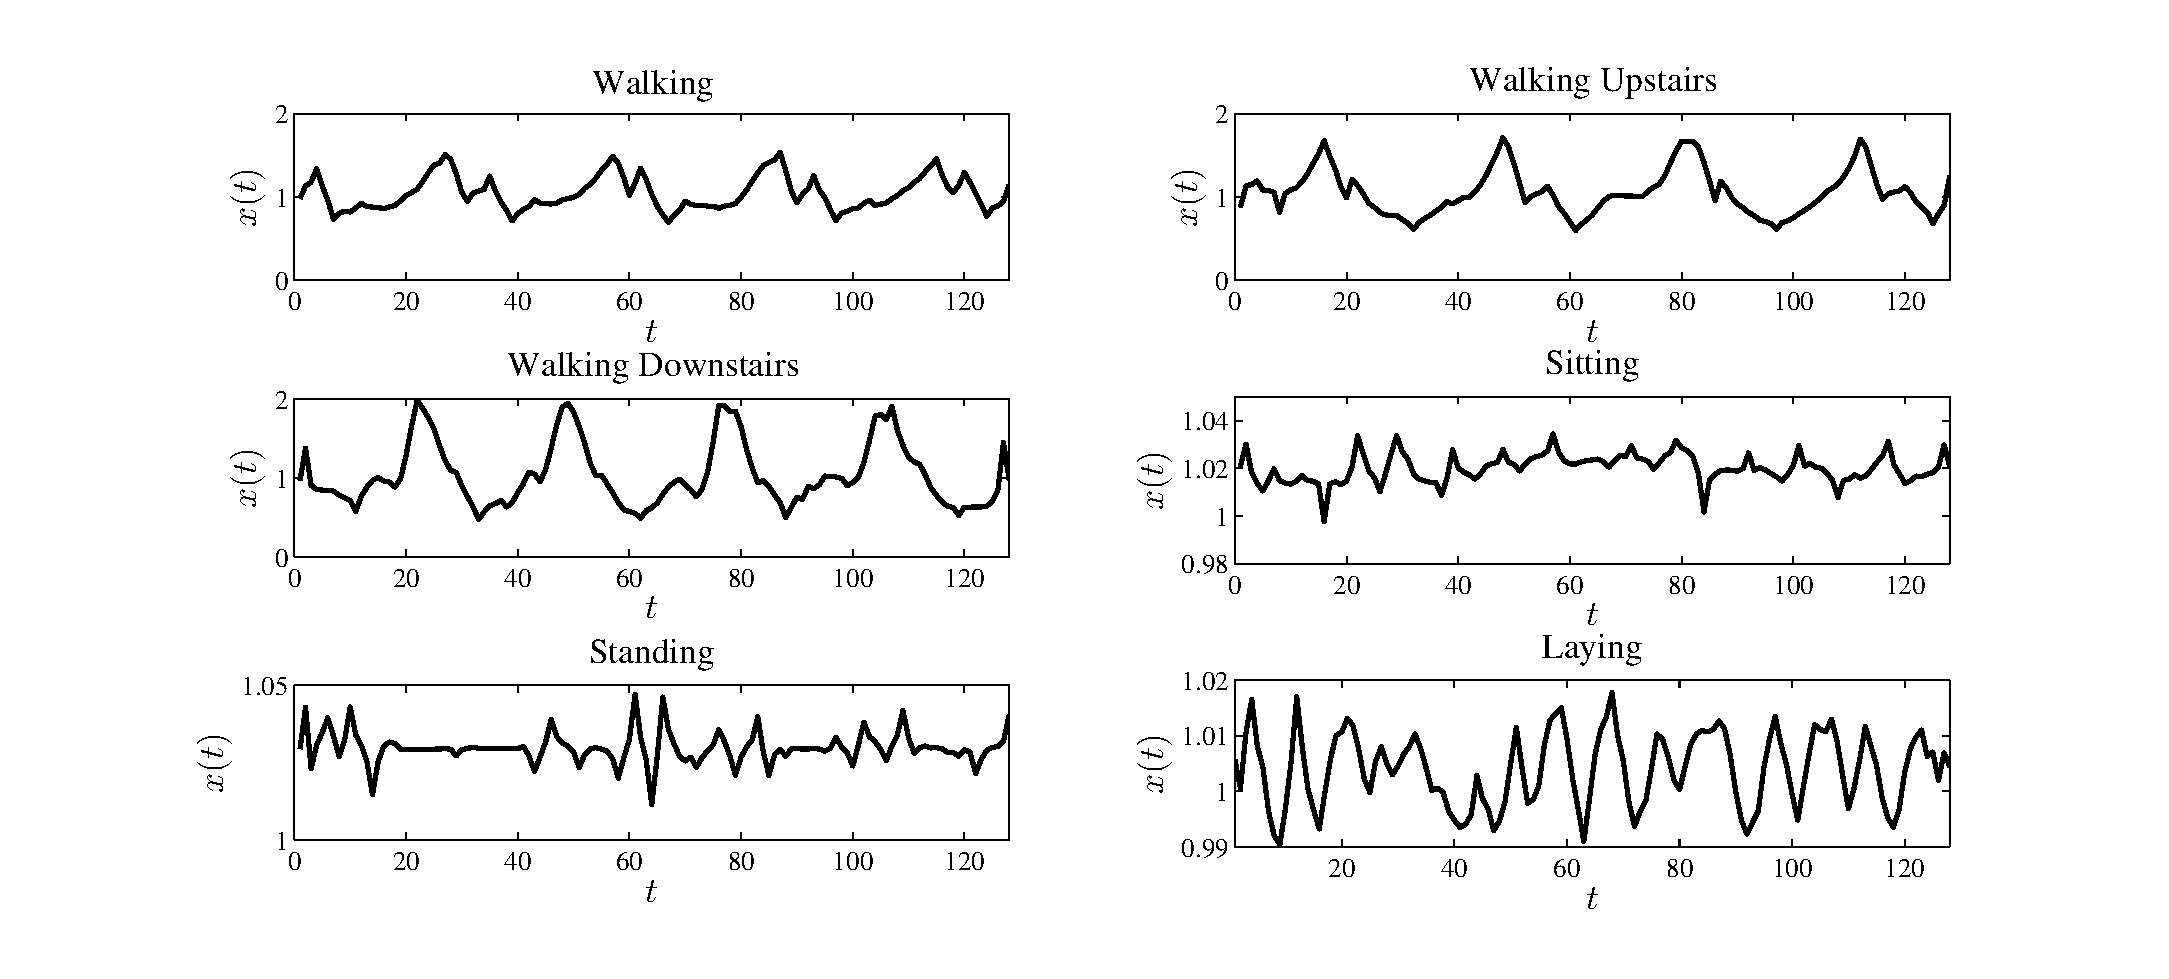
\includegraphics[width=1\linewidth]{figs/ch4/centroids_200_2}
		\caption{Центроиды временных рядов акселерометра}
		\label{centroids_real}
	\end{figure}
	На рис.~\ref{raw_ts} показаны примеры временных рядов каждого класса. Эти же временные ряды после процедуры выравнивания относительно построенных центроидов изображены на рис.~\ref{aligned_ts}.
	\begin{figure}[!ht]
		\centering
		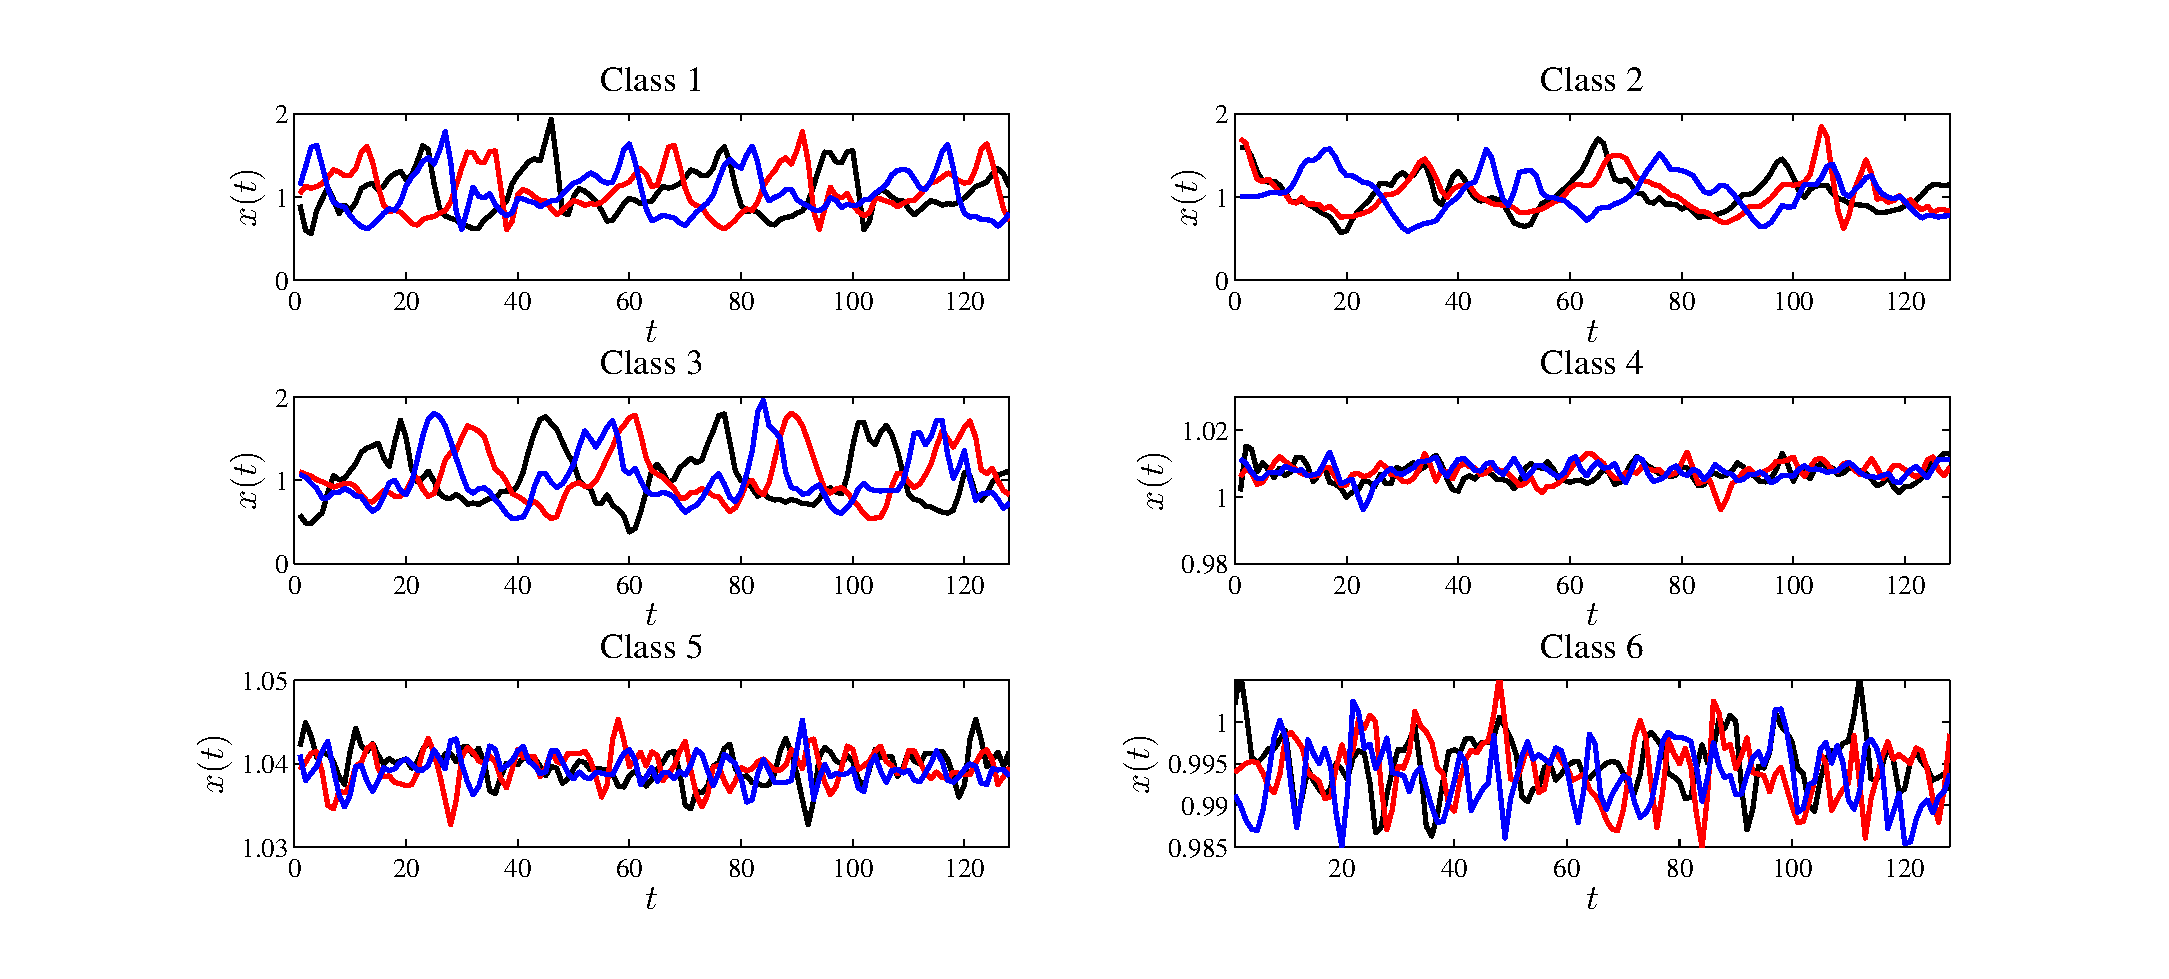
\includegraphics[width=1\linewidth]{figs/ch4/raw_ts}
		\caption{Временные ряды акселерометра}
		\label{raw_ts}
	\end{figure}
	\begin{figure}[!ht]
		\centering
		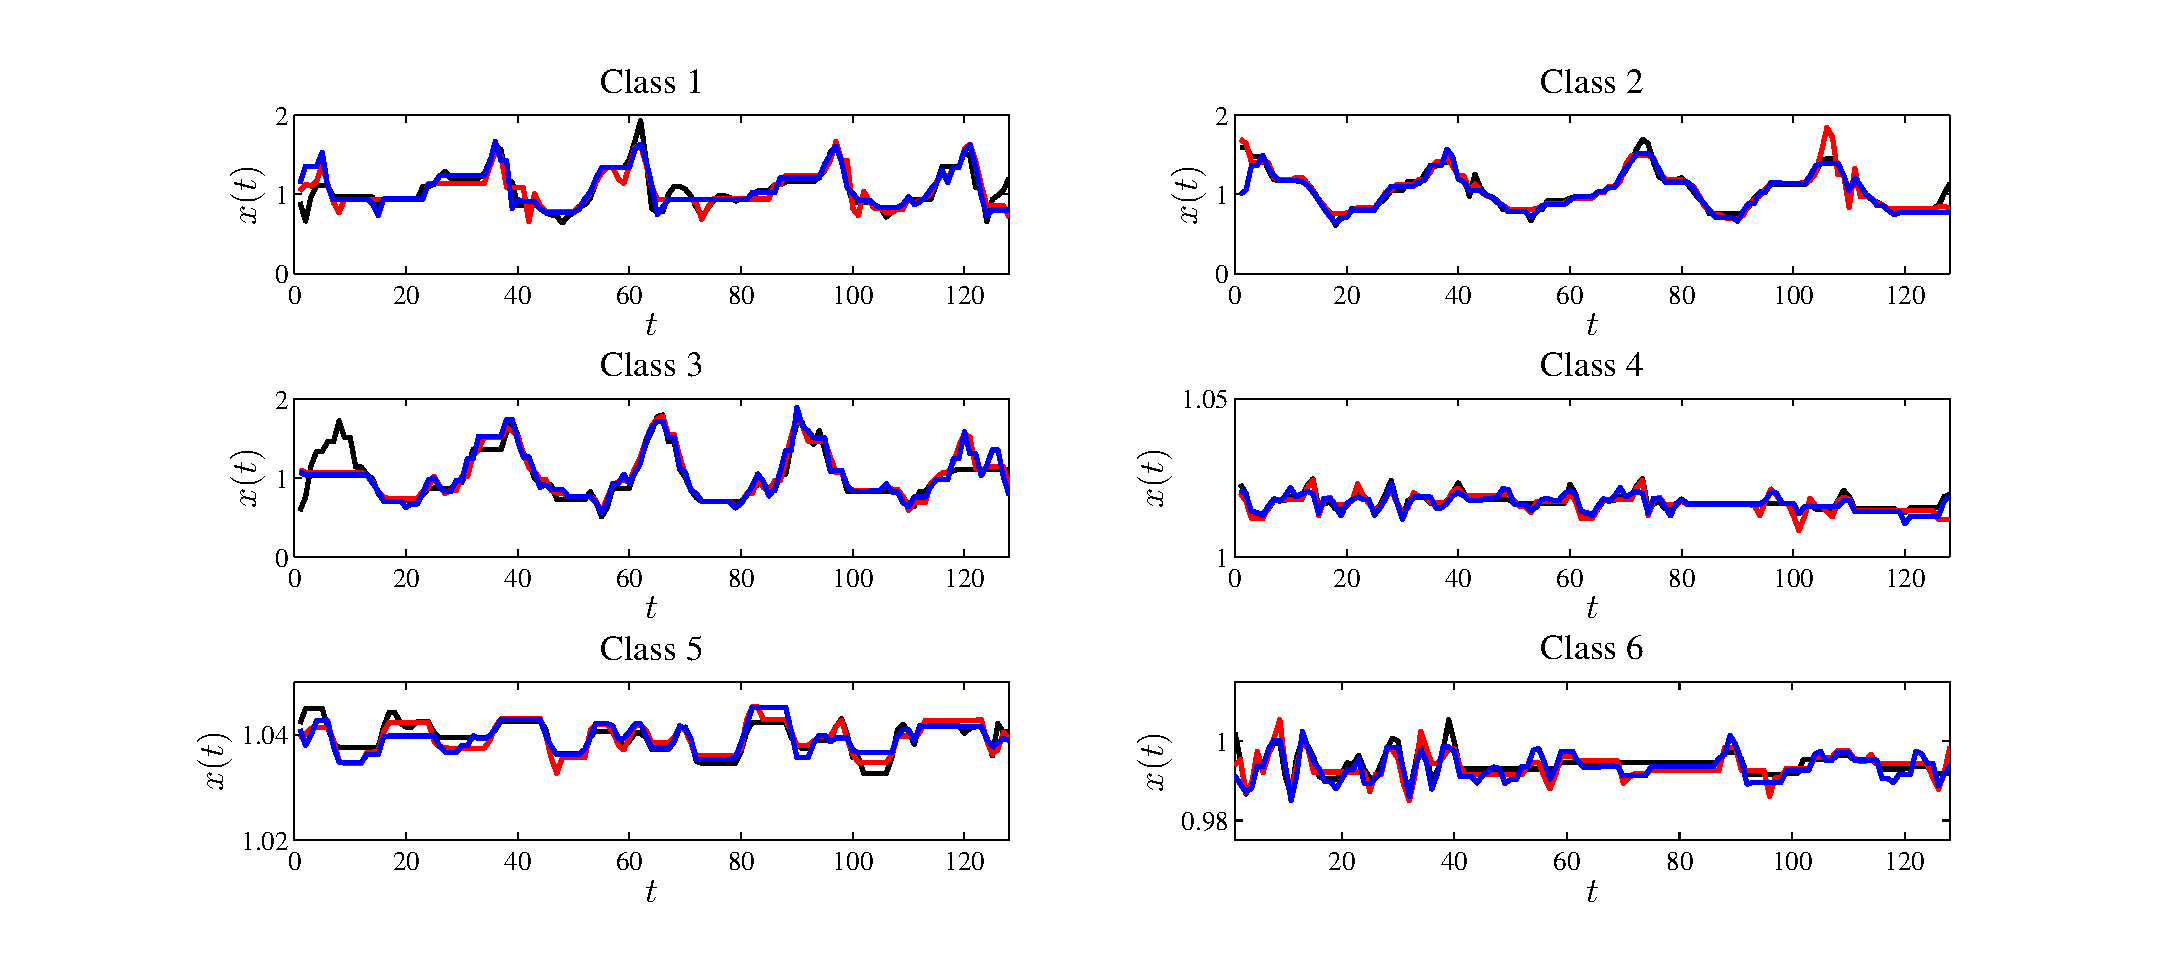
\includegraphics[width=1\linewidth]{figs/ch4/aligned_ts}
		\caption{Выравненные временные ряды акселерометра}
		\label{aligned_ts}
	\end{figure}
	
	Ошибка классификации без использования метрического обучения составила~$37,5\%$.
	Алгоритм LMNN позволяет настроить параметры: число ближайших соседей~$k$,
	размерность преобразованного евклидова пространства~$p$.
	Для выбора оптимальных параметров воспользуемся процедурой кросс-проверки.
	На рис.~\ref{heat_map} цветом показана ошибка классификации алгоритма в зависимости от его параметров.
	На данной выборке алгоритм LMNN оказывается слабо чувствителен к числу ближайших соседей,
	и при уменьшении размерности пространства объектов ошибка классификации растет.
	\begin{figure}[ht]
		\centering
		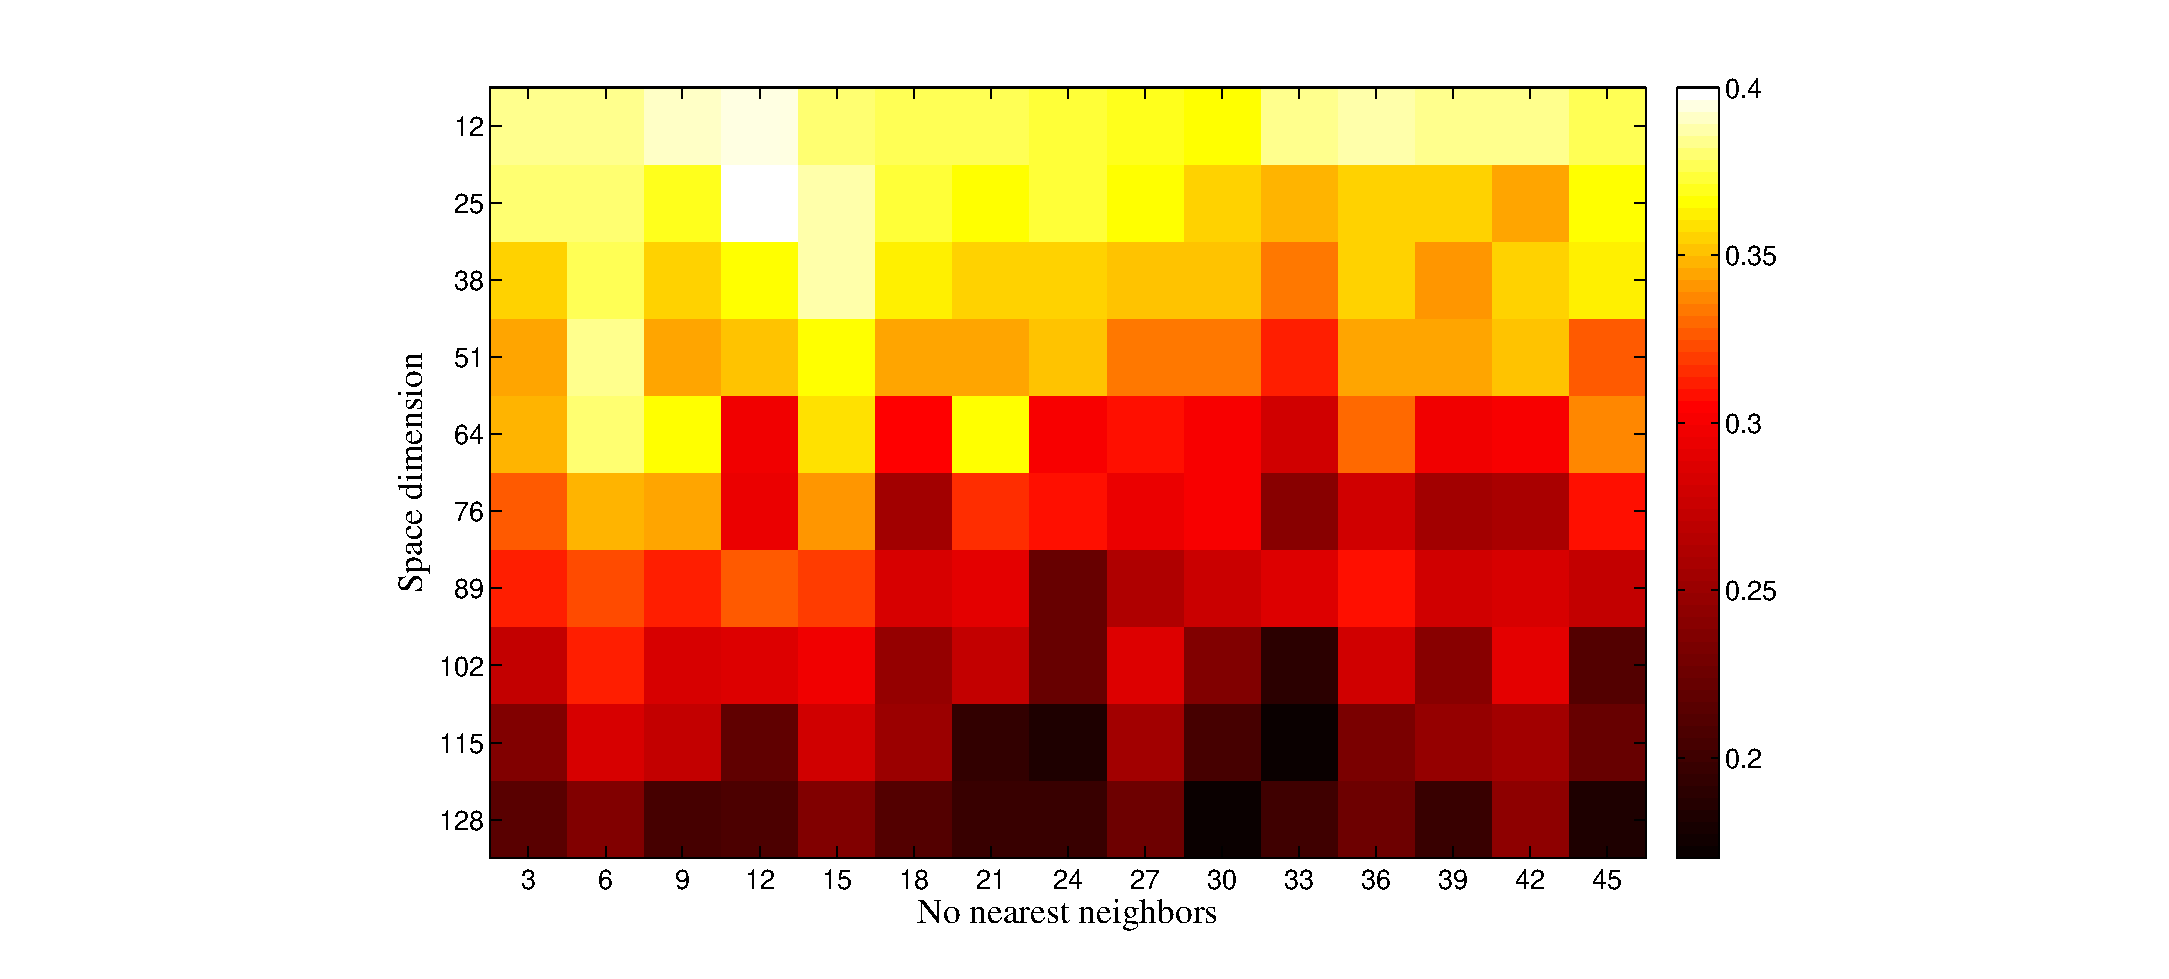
\includegraphics[width=1\linewidth]{figs/ch4/heat_map}
		\caption{Ошибка классификации в зависимости от параметров}
		\label{heat_map}
	\end{figure}
	
	Настроим алгоритм LMNN со следующими параметрами: число ближайших соседей $k = 30$, размерность
	выходного пространства $p = 128$.
	Ошибка классификации составила~$17,25\%$, что вдвое меньше ошибки классификации с использованием евклидовой метрики.
	
	\begin{table}[!ht]
		\centering
		\caption{Матрицы несоответствий}
		\subfloat[][Евклидова метрика]{\begin{tabular}{|l|l|l|l|l|l|l|}
				\hline
				\multirow{2}{*}{} & \multicolumn{6}{c|}{Истинные метки классов} \\ \cline{2-7}
				& 1     & 2     & 3     & 4     & 5    & 6    \\ \hline
				1                 & 80    & 0     & 5     & 0     & 0    & 0    \\ \hline
				2                 & 4     & 56    & 33    & 0     & 0    & 0    \\ \hline
				3                 & 5     & 5     & 86    & 0     & 0    & 0    \\ \hline
				4                 & 7     & 8     & 5     & 168   & 4    & 21   \\ \hline
				5                 & 51    & 61    & 57    & 12    & 192  & 11   \\ \hline
				6                 & 53    & 70    & 14    & 20    & 2    & 168  \\ \hline
		\end{tabular}}
		\qquad
		\subfloat[][Метрика Махаланобиса]{\begin{tabular}{|l|l|l|l|l|l|l|}
				\hline
				\multirow{2}{*}{} & \multicolumn{6}{c|}{Истинные метки классов} \\ \cline{2-7}
				& 1     & 2     & 3     & 4     & 5    & 6    \\ \hline
				1                 & 151   & 12    & 13    & 0     & 0    & 0    \\ \hline
				2                 & 10    & 142   & 14    & 0     & 0    & 0    \\ \hline
				3                 & 9     & 10    & 171   & 0     & 0    & 0    \\ \hline
				4                 & 10    & 7     & 0     & 173   & 9    & 21   \\ \hline
				5                 & 2     & 11    & 0     & 12    & 186  & 9    \\ \hline
				6                 & 18    & 18    & 2     & 15    & 5    & 170  \\ \hline
		\end{tabular}}
		\label{confussion_matrix}
	\end{table}
	
	В табл.~\ref{confussion_matrix} представлены матрицы несоответствий результатов классификации при использовании
	евклидовой метрики и метрики Махаланобиса.
	Столбцы соответствуют истинным меткам классов объектов, строки~--- предсказанным меткам.
	Диагональное преобладание матрицы несоответствий указывает на высокую предсказательную способность алгоритма.
	
	В табл.~\ref{improvement} продемонстрировано увеличение точности классификации при использовании в качестве меры расстояния метрики Махаланобиса.
	Пересечение $i$-го столбца и $j$-й строки отвечает изменению доли объектов класса $i$, отнесенных к классу $j$. Положительное суммарное значение диагональных элементов таблицы соответствует увеличению качества классификации. Значительное улучшение предсказания происходит при классификации первых трех классов.
	Данные классы соответствуют следующим видам физической активности: ходьба, ходьба вверх, ходьба вниз.
	
	\begin{table}[!ht]
		\centering
		\caption{Увеличение точности классификации при использовании адекватной оценки матрицы трансформаций}
		\label{improvement}
		\begin{tabular}{|l|l|l|l|l|l|l|}
			\hline
			\multirow{2}{*}{} & \multicolumn{6}{c|}{Истинные метки классов}       \\ \cline{2-7}
			& 1      & 2      & 3      & 4      & 5     & 6     \\ \hline
			1   & \textbf{0,355}  & 0,06   & 0,04   & 0      & 0     & 0     \\ \hline
			2   & 0,03   & \textbf{0,43}   & --0,095 & 0      & 0     & 0     \\ \hline
			3   & 0,02   & 0,025  & \textbf{0,425}  & 0      & 0     & 0     \\ \hline
			4   & 0,015  & --0,005 & --0,025 & \textbf{0,025}  & 0,025 & 0     \\ \hline
			5   & --0,245 & --0,25  & --0,28  & 0      & \textbf{--0,03} & --0,01 \\ \hline
			6   & --0,175 & --0,26  & --0,06  & --0,025 & 0,005 & \textbf{--0,01} \\ \hline
		\end{tabular}
	\end{table}
	